\newpage
\begin{section}{Integral Calculus}
	\begin{subsection}{basic integral formulas}
		$$\int \frac{1}{X} dx = \ln \vert x \vert$$
		$$\int a^{x} dx = \frac{a^x}{ln a } $$
		$$\int \sin (x) dx = -\cos (x) $$
		$$\int \cos (x) dx = \sin (x) $$
		$$\int \tan (x) dx = \ln \vert \sec (x) \vert \;\;or\;\; - \ln \vert \cos (x) \vert$$
		$$\int \cot (x) dx = \ln \vert \sin (x) \vert $$
		$$\int \sec (x) dx = \ln \vert \sec (x) + \tan (x) \vert $$
		$$\int \csc (x) dx = \ln \vert \csc (x) - \cot (x) \vert $$

	\end{subsection}
	\begin{subsection}{Weirestrass substitution}
		let $ t = \tan ( x/2 ) $ where $-\pi < x \pi $ Then:

		$$ \sin (x) = \frac{2t}{1+t^2} $$ 
		$$ \cos (x) = \frac{1-t^2}{1+t^2} $$
		$$ dx = \frac{2dt}{1 + t^2} $$
		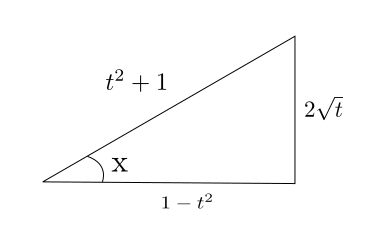
\includegraphics[]{1.png}

		if all trigonometric functions are pairs then:
		let $ t = \tan ( x ) $ where $-\pi < x \pi $ Then:


	\end{subsection}
	\begin{subsection}{Reduction formulas}
		%sen
		$$\int \sin^n (x) = - \frac{\sin^{n-1}(x)\cos(x)}{n} + \frac{n-1}{n} \int \sin^{n-2} (x) dx $$ 
		%cos
		$$\int \cos^n (x) =  \frac{\cos^{n-1}(x)\sin(x)}{n} + \frac{n-1}{n} \int \cos^{n-2} (x) dx $$ 
		%tan
		$$\int \tan^n (x) =  \frac{\tan^{n-1}(x)}{n-1}  - \int \tan^{n-2} (x) dx $$ 
		%csc
		$$\int \csc^n (x) = - \frac{\csc^{n-2}(x)\cot(x)}{n} + \frac{n-2}{n-1} \int \csc^{n-2} (x) dx $$ 
		%sec
		$$\int \sec^n (x) =  \frac{\sec^{n-2}(x)\tan(x)}{n} + \frac{n-2}{n-1} \int \sec^{n-2} (x) dx $$ 
		%cot
		$$\int \cot^n (x) =  -\frac{\cot^{n-1}(x)}{n-1}  - \int \cot^{n-2} (x) dx $$ 



		$$\int \frac{1}{(au^2 + b)^n } du = \frac{2n-3}{2b(n-1)} \int \frac{1}{(au^2 + b )^{n-1}} du + \frac{u}{2b(n-1)(au^2 + b ) ^{n-1}}$$
		$ \int \csc^n (x) \sec^n (x) dx = \frac{-\csc^{m-1} (x) \sec^{n-1} (x) } {m-1} $ $+\frac{m + n-1} {m-1} \int \csc^{m-2} (x) \sec^{n} (x) dx $

	\end{subsection}
	\begin{subsection}{integrals of Hiperbolic functions}
		$$\int \sinh (x) dx = \cosh (x) , \; \int \cosh (x) dx = \sinh (x)$$ 
		$$\int \tanh (x) dx = \ln \vert \cosh (x) \vert , \; \int \coth (x) dx = \ln \vert \sinh \vert (x)$$ 
		$$\int \sech (x) dx = \tan^{-1} (\sinh (x) ) , \; \int \csch (x) dx = \ln \vert \tanh (x) \vert $$
		$$\int \coth (x) dx = \ln \vert \sinh (x) \vert $$
	\end{subsection}
	\begin{subsection}{Particular Integrals}
$$		\int e^{\alpha x} \sin (\beta x ) dx  = [e^{\alpha x } (\alpha \sin ( \beta x ) - \beta \cos ( \beta x )) ] \frac{1}{\alpha^2 + \beta^2} $$
$$		\int e^{\alpha x} \cos (\beta x ) dx  = [e^{\alpha x } (\alpha \cos ( \beta x ) + \beta \sin ( \beta x )) ] \frac{1}{\alpha^2 + \beta^2} $$

	\end{subsection}
	\begin{subsection}{Taylor series}
		$$T(x) = \sum_{n=0}^{\infty } \frac{f^{n}(a)}{n!} (x-a)^{n}$$
	\end{subsection}
	\begin{subsection}{Riemann z function}
		$$f(s) = 1 + \frac{1}{2^5} + \frac{1}{3^5} + \frac{1}{4^5} +... $$
	\end{subsection}
	\begin{subsection}{Gamma Function}
		$$\int_{0}^{\infty} e^{-t}t^{t-1} dt = \Gamma (t) $$
		$$\gamma = \lim_{n \rightarrow \infty } [ \sum_{k=1}^{n} \frac{1}{k} - \ln (n) ] $$
	\end{subsection}
\end{section}
